\documentclass[12pt,a4paper]{article}

% Packages
\usepackage[margin=1in,left=1.5in]{geometry}
\usepackage{times}
\usepackage{setspace}
\usepackage{titlesec}
\usepackage[titles]{tocloft}
\usepackage{fancyhdr}
\usepackage{graphicx}

% Page style
\pagestyle{fancy}
\fancyhf{}
\fancyfoot[C]{\thepage}
\renewcommand{\headrulewidth}{0pt}

% Section formatting
\titleformat{\section}{\normalfont\Large\bfseries}{\thesection}{1em}{}

% Table of contents formatting
\renewcommand{\cfttoctitlefont}{\hfill\Large\bfseries}
\renewcommand{\cftaftertoctitle}{\hfill}
\renewcommand{\cftsecfont}{\normalfont}
\renewcommand{\cftsecpagefont}{\normalfont}
\setlength{\cftbeforesecskip}{5pt}

\begin{document}

% Title page
\begin{titlepage}
\begin{center}
\vspace*{2cm}
{\huge\bfseries Project Proposal\par}
\vspace{1.5cm}
{\Large\bfseries Muwaqqit\par}
\vspace{2cm}
{\Large Submitted By\par}
\vspace{1cm}
{\Large\bfseries YAZED ALKHALAF - 202211123\par}
{\Large\bfseries SAIMAN TAKLAS - 202021400\par}
{\Large\bfseries AFFAN MOHAMMAD - 202211086\par}
\vfill
{\Large Supervised By: Dr. Inaya Allah\par}
\vspace{1cm}
{\Large Al Yamamah University\par}
{\Large College of Engineering and Architecture\par}
{\Large Bachelor of Science in Software and Network Engineering\par}
\vspace{1cm}
{\Large \today\par}
\end{center}
\end{titlepage}

% Table of Contents
\tableofcontents
\clearpage

% Main content
\pagenumbering{arabic}
\doublespacing

\section{Background of the Project}

As the world is moving towards globalizing, effective time management is becoming very important. Considering how everything seems to be rushing in today's world, there is a high requirement for an effective user-friendly time management tool. Traditional calendars are used for addressing the complexities of managing multiple schedules across various aspects of life such as work, school, and personal commitments.

The introduction of the digital calendar has somewhat solved this problem but still users face a lot of issues in keeping their calendars up-to-date and synchronized. There are still few people that manually input events into their calendars. This could be real tiring dealing with multiple calendars.

Moreover, the rise of instant messaging platforms like WhatsApp has changed the way we communicate and plan events. Mostly, important dates and appointments are discussed informally leading to a disconnect between where the information is initially shared and where it needs to be recorded for effective time management. 

\section{Problem Statement}

The core problem that Muwaqqit addresses is the inefficient and potential conflicts in managing the personal and professional schedules in a globalized world, especially:

\begin{enumerate}
    \item Users struggle to keep their calendars up-to-date with information from various sources, particularly form informal modes of communication such as WhatsApp.
    \item They manually add the events to the calendar which is time consuming and complex.
    \item Multiple calendars (work, school and personal) create complexity and major risk of conflicts.
    \item There is a lack of seamless integration with popular communication platforms.
    \item High risk of missing events due to various distribution of information in other calendars.
\end{enumerate}

\section{Objectives of the Project}

The main objectives of Muwaqqit are:

\begin{itemize}
    \item To develop an intelligent calendar management system that automatically extracts events from the communication channels and adds to the user's main calendar.
    \item To create a user friendly interface that allows users to automatically add events to the calendar.
    \item To implement smart resolution system that notifies users of scheduling conflicts and provides easy options for resolution.
    \item To integrate all the calendars into Muwaqqit's single calendar to make managing all the events easy.
    \item To block/hold the calendar for daily routines such as waking time, sleeping time and prayer time.
    \item To significantly reduce the time users spend on manual calendar management.
\end{itemize}

\section{Significance of the Project}

Muwaqqit endeavours to solve problems and its significance can be summarized in the following:

\begin{enumerate}
    \item \textbf{Time is Money}: Time is the only asset you can't get more of, it is being consumed til the last day of your life.
    \item \textbf{Prayer First Calendar}: Prayer times come first, then your daily scheduled items.
\end{enumerate}

\section{Scope of the Project}

We aren't a calendar, we just aggregate your calendar and your data sources to make your life easier.

\section{Limitations of the Project}

Nothing is perfect, and our project is not a outlier. The limitations we have figured out about it are as follows:

\begin{itemize}
    \item WhatsApp integration allows the app to read the users messages, so it would be hard to prove privacy hasn't been breached.
    \item WhatsApp integration might not always be there, they are a third-party and we will be using a non-official integration path.
    \item Learning new languages and technologies for the project might need more time than we aniticipate.
    \item Accuracy of our algorithms to detect keywords indicating an event agreement has happenned, especially for languages other than English and Arabic.
\end{itemize}

\section{Project Plan}

Our project plan can be illustrated in the following gantt chart, \textbf{Figure \ref{fig:project-gantt-chart}}.

\begin{figure}[!h]
    \centering
    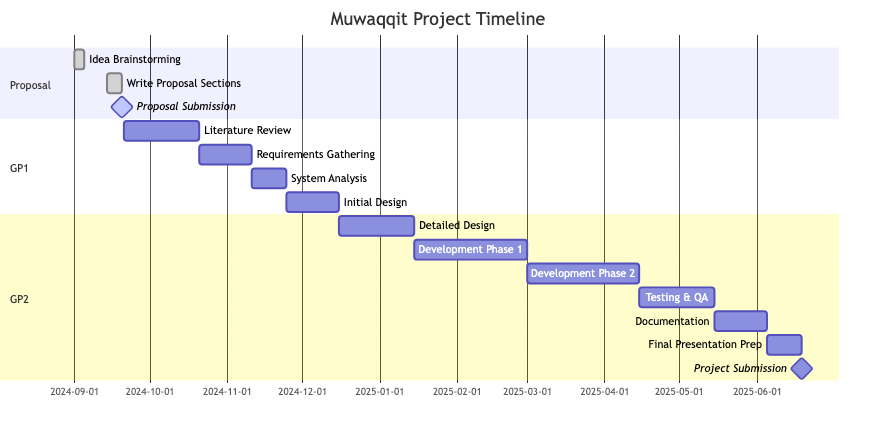
\includegraphics[width=\textwidth]{images/gantt.png}
    \caption{Project Gantt Chart}
    \label{fig:project-gantt-chart}
\end{figure}

\section{Literature Review}

In developing Muwaqqit, we have drawn inspiration from and built upon existing research and products in the field of intelligent calendar management. Some key references include:

\begin{itemize}
    \item \textbf{Clockwise (https://www.getclockwise.com/):} An AI-powered calendar assistant that optimizes schedules and manages team coordination. Clockwise's approach to intelligent time blocking and meeting optimization provides valuable insights for Muwaqqit's AI-driven features.
    \item \textbf{An Exploratory Study of Calendar Use:} "Prospective remembering is the use of memory for remembering to do things in the future, as different from retrospective memory functions such as recalling past events."
\end{itemize}

\section{Conclusion}

\end{document}